\section{Results and Discussion}
% do they want p-values and stuff? like does that make sense in this context? i.e. is this binary predictor better than this one.\


\subsection{Classifier Accuracy}
The canonical Na\"ive Bayes (NB)\nomenclature{NB}{Na\"ive Bayes} and Decision Tree (DT)\nomenclature{DT}{Decision Tree} classification algorithms were implemented with tie decisions resulting in a `yes' and are hereafter referred to as MyNB and MyDT respectively. 10-fold stratified cross validation was then performed on these algorithms and 12 other inbuilt Weka algorithms using the dataset described in section \ref{sec:data} after normalisation and discretisation for the numeric and nominal classification algorithms respectively.

Tables \ref{tab:acc:num} and \ref{tab:acc:nom} present all the resulting accuracy figures for each tested classification algorithm, shown in percentage (\%) to 4 d.p.\nomenclature{d.p. decimal points} , using both the full dataset and the dataset after CFS, and coloured for ease of comparison.

\begin{table}[h]
    \caption{The 10-fold stratified cross validation accuracy in percentage (\%) of each tested \textit{numeric} classification algorithm using the dataset with and without CFS. \label{tab:acc:num}}
    \begin{center}
    \begin{tabular}{|m{2cm}*{8}{|R}|}
        \hline
        \textbf{Numeric Data} & ZeroR\nomenclature{ZeroR}{Classifier that always predicts the majority class} & 1R\nomenclature{1R}{One Rule} & 1NN\nomenclature{kNN}{k-Nearest Neighbours} &5NN &NB &MLP\nomenclature{MLP}{Multilayer Perceptron} &SVM\nomenclature{SVM}{Support Vector Machines} & \color{blue}MyNB \EndTableHeader \\
        \hline
        No feature selection & 65.1042 &70.8333 &67.8385 &74.4792 &75.1302 &75.3906 &76.3021 &75.2614 \\
        \hline
        CFS & 65.1042 &70.8333 &69.0104 &74.4792 &76.3021 &75.7813&76.6927 & 76.0407 \\
        \hline
    \end{tabular}
    \end{center}
\end{table}

\begin{table}[h]
    \caption{The 10-fold stratified cross validation accuracy in percentage (\%) of each tested \textit{nominal} classification algorithm using the dataset with and without CFS. \label{tab:acc:nom}}
    \begin{center}
    \begin{tabular}{|m{2cm}*{6}{|R}|}
        \hline
        \textbf{Nominal Data} & DT unpruned &DT pruned &\color{blue}MyDT &Bagg\nomenclature{Bagg}{Bagging} &Boost\nomenclature{Boost}{Boosting} &RF\nomenclature{RF}{Random Forest} \EndTableHeader \\
        \hline
        No feature selection &75.0000 & 75.3906 &73.4484 &74.8698&76.1719&73.1771 \\
        \hline
        CFS & 79.4271 & 79.4271 &78.3869 & 78.5156 & 78.6458 & 78.9063 \\
        \hline
    \end{tabular}
    \end{center}
\end{table}

\subsection{DT Diagrams}
Decision trees were built on the full discretised dataset using three different algorithms: MyDT, and two DT classifiers from Weka (DT unpruned and DT pruned). The MyDT tree was built using the ID3 algorithm (without pruning), which recursively builds a tree based on maximum information gain. The two Weka variants were built using J48 (an implementation of the C4.5 algorithm) with default parameters, but differ in that one has been pruned in addition to the other \cite{weka}. The DT diagrams are displayed in Figures \ref{fig:mydt}, \ref{fig:dt_unprune} and \ref{fig:dt_prune} in section \ref{sec:dix}.

\subsection{Discussion}
% kinda tempted to change structure? like combine DT diagrams with DT here idk

\subsubsection{Comparison of Classifiers}
% for that extra WOW we could have a bar chart or something?

% In the discussion, compare the performance of the classifiers, with and without feature selection. Compare your implementations of NB and DT with Weka’s.

Overall, the accuracy of the 14 classifiers ranged roughly between 65\% and 80\% with a mean of $\sim$74.5\%. \\

The best performing numeric classifier was the SVM, both with and without feature selection, where it achieved an accuracy of $\sim$76.7\% and $\sim$76.3\% respectively. Similar in performance were MyNB, NB and MLP, with accuracies roughly within 1\% of the SVM. This small difference in accuracies ranging from 75\% to 77\% is not necessarily indicative of algorithmic superiority but may be the effect of random noise in the testing dataset.

On the other hand, the worst performing numeric classifiers were ZeroR, 1R and 1NN, achieving accuracies between 65\% and 71\%. These simple algorithms are clearly not complex enough to capture patterns in the data, but are instead good points for comparison as to what is easily achievable (for example by predicting the majority class in ZeroR).

Within the nominal classifiers, the highest accuracy was $\sim$79.4\%, and was obtained by both the pruned and unpruned DT using feature selection. Despite this, all of the nominal classifiers performed well using feature selection, with accuracies ranging roughly between 78\% and 79.5\%. Without feature selection, the best performing nominal classifier was Boost with an accuracy of $\sim$76.2\%.

The worst performing nominal classifier was MyDT, with and without feature selection, where it achieved an accuracy of $\sim$78.3\% and $\sim$73.4\% respectively.
\\

The 6 nominal classifiers clearly performed much better than the 8 numeric ones with a mean accuracy of $\sim$76.8\% compared to $\sim$72.8\%. In addition, using CFS improved or equalled the performance of every classifier, with an average improvement in accuracy of $\sim$2.1\%. \\


The implementations of MyNB and Weka's NB only differ in terms of their running time performance. In fact, the minimal differences in accuracies evident in Table \ref{tab:acc:num} are most likely the result of different 10-fold data stratifications used in the cross validation accuracy calculations. On the other hand, the implementations of MyDT and Weka's two DTs differ profoundly. MyDT is built using the ID3 algorithm without pruning, whilst Weka uses J48 (an implementation of the 8th revision of the C4.5 algorithm \cite{weka}) which is very similar to ID3 but using the normalised information gain ratio as its splitting criterion. This resulted in Weka's two DTs performing better than MyDT with and without feature selection.


\subsubsection{Feature Selection}

% Discuss the effect of the feature selection – did CFS select a subset of the original features, and if so, did the selected subset make intuitive sense to you? Was the feature selection beneficial, i.e. did it improve accuracy, or have any other advantages? Why do you think this is the case?

The feature selection method (CFS) selected a subset of 5 features from the original 9. As is highlighted in Table \ref{tab:cols}, these were, in no particular order:

\begin{itemize}
    \item Plasma glucose concentration
    \item Serum insulin level
    \item BMI
    \item Diabetes pedigree function
    \item Age
\end{itemize}

It makes sense that this selected subset is highly correlated with the onset of diabetes but also mutually uncorrelated. \\

In fact, having diabetes is defined for the dataset in question as obtaining a plasma glucose concentration of at least 200 mg/dL, 2 hours after the ingestion of 75mg of carbohydrate solution \cite{pima}. So it is no surprise that CFS claims that glucose concentration is a strong predictor of the onset of diabetes. Furthermore, the level of insulin has been found to be one of the strongest predictors of the onset of diabetes in numerous studies containing a wide range of attributes \cite{a,b,c,d}. Although glucose concentration and insulin levels often exhibit a significant inversely-correlated relationship when measured via an oral glucose tolerance test (OGTT)\nomenclature{OGTT}{Oral glucose tolerance test} and insulin release test (IRT)\nomenclature{IRT}{Insulin release test} respectively \cite{e}, the original dataset description is vague as to how the insulin level was recorded. In fact, Figure \ref{fig:corr} shows that all of the 5 selected attributes in the CFS subset are mutually uncorrelated, as expected.

Furthermore, BMI and other weight-related features have also previously been found to be good predictors of the onset of diabetes \cite{a,c,d}. Specifically within our dataset, the weight-related features are BMI and triceps skin fold thickness, which are known to be significantly correlated \cite{f}. However, BMI has a higher association with health-related risk factors than triceps skin fold thickness \cite{g,h}, which explains why it was prioritised in the CFS subset.

The two other features selected by CFS are also known to have a high correlation with diabetes. In particular, age has been shown to be both a strong predictor \cite{i} and also relatively uncorrelated with other features, as demonstrated by its inclusion in principal component analysis (PCA)\nomenclature{PCA}{Principal component analysis} in a different paper using the same dataset \cite{c}. Family history of diabetes has also been shown to be a relatively strong and independent predictor of diabetes \cite{j}. \\

\begin{figure}[htp] \centering{
    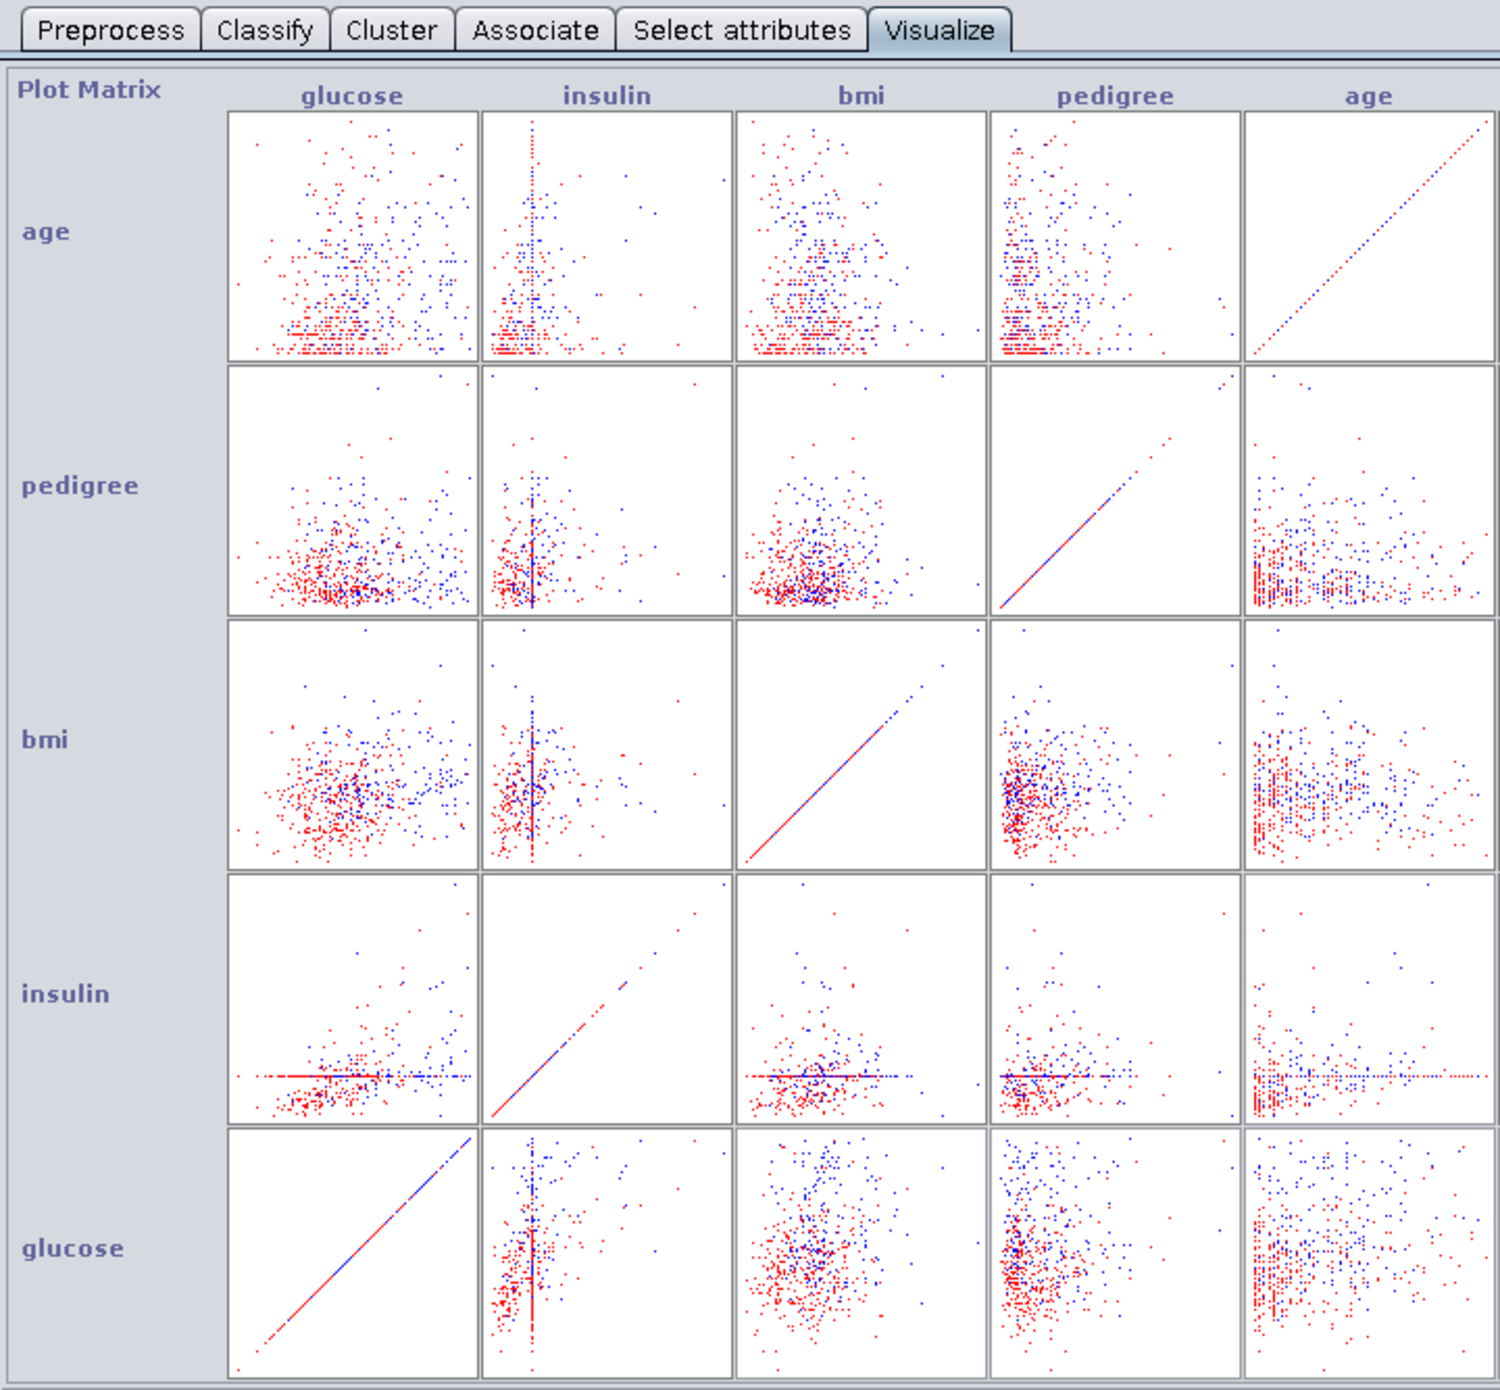
\includegraphics[scale=0.75]{corr.pdf}}
\caption{Scatter plot matrix using Weka with each variable from CFS.\label{fig:corr}}
\end{figure}

% then show it was better / other advantages (speed, memory). state why.

Across all models, the accuracy either improved or stayed the same after using CFS compared to no feature selection, with an average improvement in accuracy of $\sim$2.1\%. This effect was most apparent with tree-based models, with the accuracy improving by $\sim$5\% for DT pruned and unpruned, MyDT and RF. This is likely due to a reduction in over fitting, stemming from the removal of features that did not add much information or were otherwise terrible predictors of the onset of diabetes.

Another advantage of CFS is the reduction in memory size and computational time. This is especially noticeable when pruning large datasets that have many features which are highly correlated with each other  or poorly correlated with the target classification. In our dataset for example, the number of features was reduced by over 40\%. Not only does this allow for smaller file sizes and therefore faster training and testing, but it can also increase the interpretability of models as there are less features being used when visualising decision trees.

\subsubsection{Decision Trees}
\label{sec:dis_dt}

% How does your DT classifier compare with the unpruned and pruned DT generated by Weka? Discuss the role and effect of pruning.
% Comparison between the DT classifiers and discussion of pruning
 
Although all three decision tree algorithms (MyDT, DT unpruned and DT pruned) differ in both the method used and 10-fold accuracy, each algorithm uses a splitting method that tends to reduce the information entropy of the partitioned data. As a result, we see strong similarities in the first couple splits of each tree. In particular, the diagrams in section \ref{sec:dix} reveal that each tree found glucose to be the best feature to first split on, as its high correlation with diabetes caused it to produce in the largest reduction in information entropy compared to other features. The second splits are also quite similar, with each tree subsequently splitting on either BMI, insulin, or age, depending on the value of the parent glucose attribute.

After a few splits however, slight differences in the algorithms start to become apparent in the tree diagrams. For one, Weka's J48 DT with pruning (Figure \ref{fig:dt_prune}) reaches leaf nodes on the third and fourth split, whereas Weka's unpruned J48 tree (Figure \ref{fig:dt_unprune}) generally continues until split six or seven. In comparison, our unpruned ID3 implementation (Figure \ref{fig:mydt}) reaches 8 splits in some cases. Interestingly, the depth of the tree seems to be directly negatively correlated with the relative performance of the algorithm. This is likely due to the presence of over-fitting that occurs when you begin splitting on smaller and smaller partitions of the original data, causing the tree to start splitting on noise rather than patterns.

One method to prevent such over-fitting, as implemented by Weka's best performing J48 tree, is the powerful concept of pruning. This strategy involves iteratively removing leaf nodes from a tree by replacing the sub-tree from which a family of leaves stem with a new leaf node, that then classifies as the majority of class of that subtree. At each step, the new validation accuracy of the resulting tree is compared and the process is repeated until all subtree reductions result in a loss of accuracy. As clear with the superior performance of the pruned J48 tree, such a procedure can allow the size of a tree to be significantly reduced whilst simultaneously increasing overall accuracy.


\subsubsection{Tree-based Ensemble Classifiers}

% Comparison between the tree-based classifiers
% Compare the accuracy of the tree-based classifiers (DT, Bagging, Boosting and RF).

Although tree-based classifiers exist for numeric features, our study focuses on the use of tree-based classifiers for exclusively nominal data. Out of the six tree-based classifiers tested, three are variations of single decision trees (discussed in section \ref{sec:dis_dt}), and the other three use ensemble methods. Ensemble methods involve the creation of a number of single classifiers, where each classifier makes a prediction, and the results are combined similar to a voting mechanism. As we are combining multiple predictions from different classifiers, ideally, the mistakes made by one classifier will be outvoted by the predictions from other classifiers which are correct on those particular samples. In the case of our study, the ensemble methods tested were bagging, boosting, and random forest.

Bagging involves `bootstrapping' a number of new datasets by sampling from the original data with replacement, and then distributing the bootstrapped datasets among a number of single classifiers for training. Predictions on new data are then calculated by combining the predictions from each classifier through a majority vote with equal weighting. While bagging did have some improvements over MyDT and RF without feature selection, this particular ensemble method did not prove particularly beneficial in predicting diabetes over single J48 trees.

Boosting was the second ensemble method used in our study. This involves creating a series of classifiers, where the data of the next classifier is weighted towards the misclassified examples in the previous classifier. Unlike bagging, individuals trees are then given different weighting in the final vote for new predictions, typically depending on their overall performance on the training data. In our study, boosting performed particularly well on the dataset without feature selection, as it beat the second best tree-based classifier by almost 1\%. Interestingly, this advantage diminished after CFS was applied.

The last ensemble method used was Random Forest. In contrast to boosting, this method was the worst tree-based method without feature selection, but outperformed both bagging and boosting after CFS was applied. Similar to bagging, this algorithm generates multiple new datasets which are then distributed among single trees for training and majority-vote predictions subsequently. The key difference being that random forests use a random subset of the original features, rather than sampling from individual examples.


% \subsubsection{?Anything else that we consider important}
% % Include anything else that you consider important

% Nominal better? Weird?? Discussion point?
% or is the data being predicted here actually different? if not its probs just overfitting (to noise) or something when given more DOF(?) and thats something to mention.


% could also talk about why J48 DT is the best. again, look into specifics of J48 and try to justify that it had all advantages of DT without disadvantages (+ advantages that other algos had).
